% Created 2024-10-16 śro 21:35
% Intended LaTeX compiler: pdflatex
\documentclass[../../main.tex]{subfiles}

\usepackage[T1]{fontenc}
\usepackage[utf8]{inputenc}
\usepackage{graphicx}
\usepackage{longtable}
\usepackage{wrapfig}
\usepackage{rotating}
\usepackage[normalem]{ulem}
\usepackage{amsmath}
\usepackage{capt-of}
\usepackage{hyperref}
\usepackage{siunitx}
\usepackage{float}
\usepackage[polish]{babel}

\graphicspath{{../}}
\author{Wojciech Paderewski}
\date{\today}
\title{Koncepcja ukladu}
\hypersetup{
 pdfauthor={Wojciech Paderewski},
 pdftitle={Koncepcja ukladu},
 pdfkeywords={},
 pdfsubject={},
 pdflang={Polish}}
 
\begin{document}
Przetwornica impulsowa wysokiego napięcia jest najtrudniejszym do zaprojektowania elementem układu.
Ma ona posiadać regulowane programowo napięcie wyjściowe, co dodatkowo komplikuje projekt.
Nie może być również użyta zbyt duża cewka, ponieważ celem jest stworzenie niskiego urządzenia.

\subsubsection{Założenia projektowe}
\begin{itemize}
    \item Napięcie wejściowe: \SI{12}{\volt}
    \item Napięcie wyjściowe: 130-220 V
    \item Prąd wyjściowy: \SI{20}{\milli\ampere}
    \item \SI{0.1}{\volt} tętnienia napięcia wyjściowego
\end{itemize}

\subsubsection{Wybór układu scalonego}
Wybrano układ LM3488 produkcji Texas Instruments, który jest układem przeznaczonym do budowy przetwornic typu Boost oraz Flyback. 
Jest to układ high efficiency, co jest powodem dla którego został wybrany \cite{st:lm3488}.

Jako początkowe założenie przyjęto częstotliwość przełączania \SI{400}{\kilo\hertz} zgodnie z domyślną wartością w nocie katalogowej układu, 
ale możliwe jest zwiększanie częstotliwości do \SI{1}{\mega\hertz}, co pozwala na zmniejszenie rozmiarów cewki oraz kondensatorów, natomiast może to
pogorszyć sprawność układu, ponieważ według karty katalogowej wraz ze wzrostem częstotliwości spada wzmocnienie układu, co przekłada się na mniejszą sprawność.
Podczas projektowania wzorowano się na schemacie z karty katalogowej, który przedstawiono na rysunku \ref{fig:boost}.

\begin{figure}[H]
    \centering
    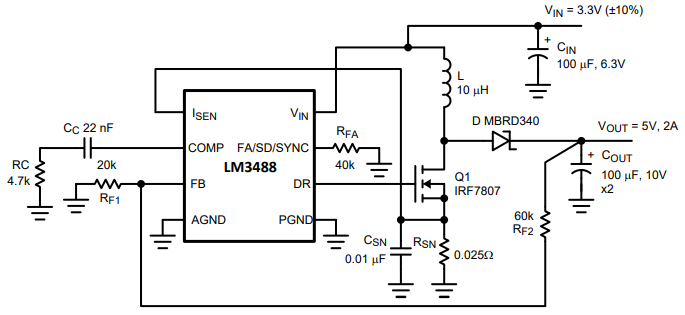
\includegraphics[width=0.8\textwidth]{boost.png}
    \caption{Schemat układu z karty katalogowej \cite{st:lm3488}}
    \label{fig:boost}
\end{figure}

\subsubsection{Dobór cewki}
Wartość prądu cewki oszacowano na podstawie założonego prądu wyjściowego:

\begin{equation}
    I_{l} = \frac{V_{out} \cdot I_{out}}{V_{in}} = \frac{220 \cdot 0.02}{12} \approx \SI{0.36}{\milli\ampere}
\end{equation}

Dodatkowe 30\% prądu wyjściowego zostało dodane jako tętnienia prądu, co pozwala oszacować wartość maksymalnego prądu cewki:
\begin{equation}
    I_{peak} = (1+0.3) \cdot I_{l} = 1.3 \cdot 0.36 \approx \SI{0.468}{\ampere}
\end{equation}

Wynika z tego, że potrzebna jest cewka o prądzie przewodzenia większym niż \SI{0.5}{\ampere}.

Obliczono wypełnienie sygnału PWM, na podstawie wzoru:
\begin{equation}
    D_{220} = \frac{V_{out}-V_{in}}{V_{out}} = \frac{220-12}{220} \approx 0.945
\end{equation}

\begin{equation}
    D_{130} = \frac{V_{out}-V_{in}}{V_{out}} = \frac{130-12}{130} \approx 0.908
\end{equation}

Zgodnie z kartą katalogową układu LM3488, cewka powinna mieć wartość określaną wzorem:
\begin{equation}
    L > \frac{D(1-D)V_{in}}{2f_{sw}I_{out}}
\end{equation}

Według dokumentacji $I_{out}$ podczas obliczeń powinno stanowić 30\% minimalnej wartości prądu wyjściowego:
\begin{equation}
    I_{out} = 0.3 \cdot \SI{20}{\milli\ampere} = \SI{6}{\milli\ampere}
\end{equation}

Dla napięcia wyjściowego \SI{220}{\volt} oraz napięcia wejściowego \SI{12}{\volt} oraz częstotliwości \SI{400}{\kilo\hertz} otrzymano wartość cewki:
\begin{equation}
    L_{220} > \frac{0.945 \cdot (1-0.945) \cdot 12}{2 \cdot 400000 \cdot 0.006} \approx \SI{128.9}{\micro\henry}
\end{equation}

Natomiast dla napięcia wyjściowego 130\si{\volt} oraz napięcia wejściowego \SI{12}{\volt} oraz częstotliwości \SI{400}{\kilo\hertz} otrzymano wartość cewki:
\begin{equation}
    L_{130} > \frac{0.908 \cdot (1-0.908) \cdot 12}{2 \cdot 400000 \cdot 0.006} \approx \SI{209.5}{\micro\henry}
\end{equation}

Napotkano problem z doborem cewki, ponieważ nie udało się znaleźć w sklepie cewki o wartości powyżej \SI{200}{\micro\henry} w rozsądnej cenie i odpowiednich rozmiarach.
Dlatego zdecydowano się na zastosowanie cewki o wartości \SI{180}{\micro\henry}, która jest najbliższą wartością dostępną w sklepie. Wartość
graniczna prądu cewki wynosi \SI{0.9}{\ampere}, co jest wystarczającym zapasem. Wybrana cewka ma rezystancję \SI{6.3}{\milli\ohm}.
Moc strat w cewce wynosi:

\begin{equation}
    P_{l} = I_{peak}^2 \cdot R = 0.468^2 \cdot 0.0063 \approx \SI{1.4}{\milli\watt}
\end{equation}

W celu osiągnięcia założonego zakresu napięcia wyjściowego z użyciem wybranej cewki, zdecydowano się na zwiększanie częstotliwości przełączania do \SI{500}{\kilo\hertz}.
Obliczono wartość cewki dla napięcia wyjściowego \SI{130}{\volt} oraz napięcia wejściowego \SI{12}{\volt} oraz częstotliwości \SI{500}{\kilo\hertz}:
\begin{equation}
    L_{220} > \frac{0.945 \cdot (1-0.945) \cdot 12}{2 \cdot 500000 \cdot 0.006} \approx \SI{103.1}{\micro\henry}
\end{equation}
\begin{equation}
    L_{130} > \frac{0.908 \cdot (1-0.908) \cdot 12}{2 \cdot 500000 \cdot 0.006} \approx \SI{167.6}{\micro\henry}
\end{equation}
Z obliczeń wynika, że zwiększanie częstotliwości pozwala na zmniejszenie wartości cewki, co pozwala na zastosowanie cewki o wartości \SI{180}{\micro\henry}.

\subsubsection{Dobór kondensatorów}
Według zaleceń z karty katalogowej w przetwornicy powinny być zastosowane kondensatory o jak najniższym ESR,
dlatego odrzucono kondensatory elektrolityczne na rzecz kondensatorów ceramicznych, które mają bardzo niski ESR, tak
mały że producent nie podaje tej wartości w notach katalogowych, gdyż jest ona zbyt mała by miała znaczenie.

Jednak problemem jest znalezienie kondensatorów ceramicznych pracujących przy wysokim napięciu, mimo tego został znaleziony kondensator 
ceramiczny o wartości \SI{2.2}{\micro\farad} i napięciu pracy do \SI{250}{\volt}.

W obliczeniach należy uwzględnić spadek pojemności kondensatora wraz ze wzrostem napięcia.
Wartości spadku pojemności dla kondensatora ceramicznego odczytano z \cite{st:ceramic-capacitor}.
\begin{figure}[H]
    \centering
    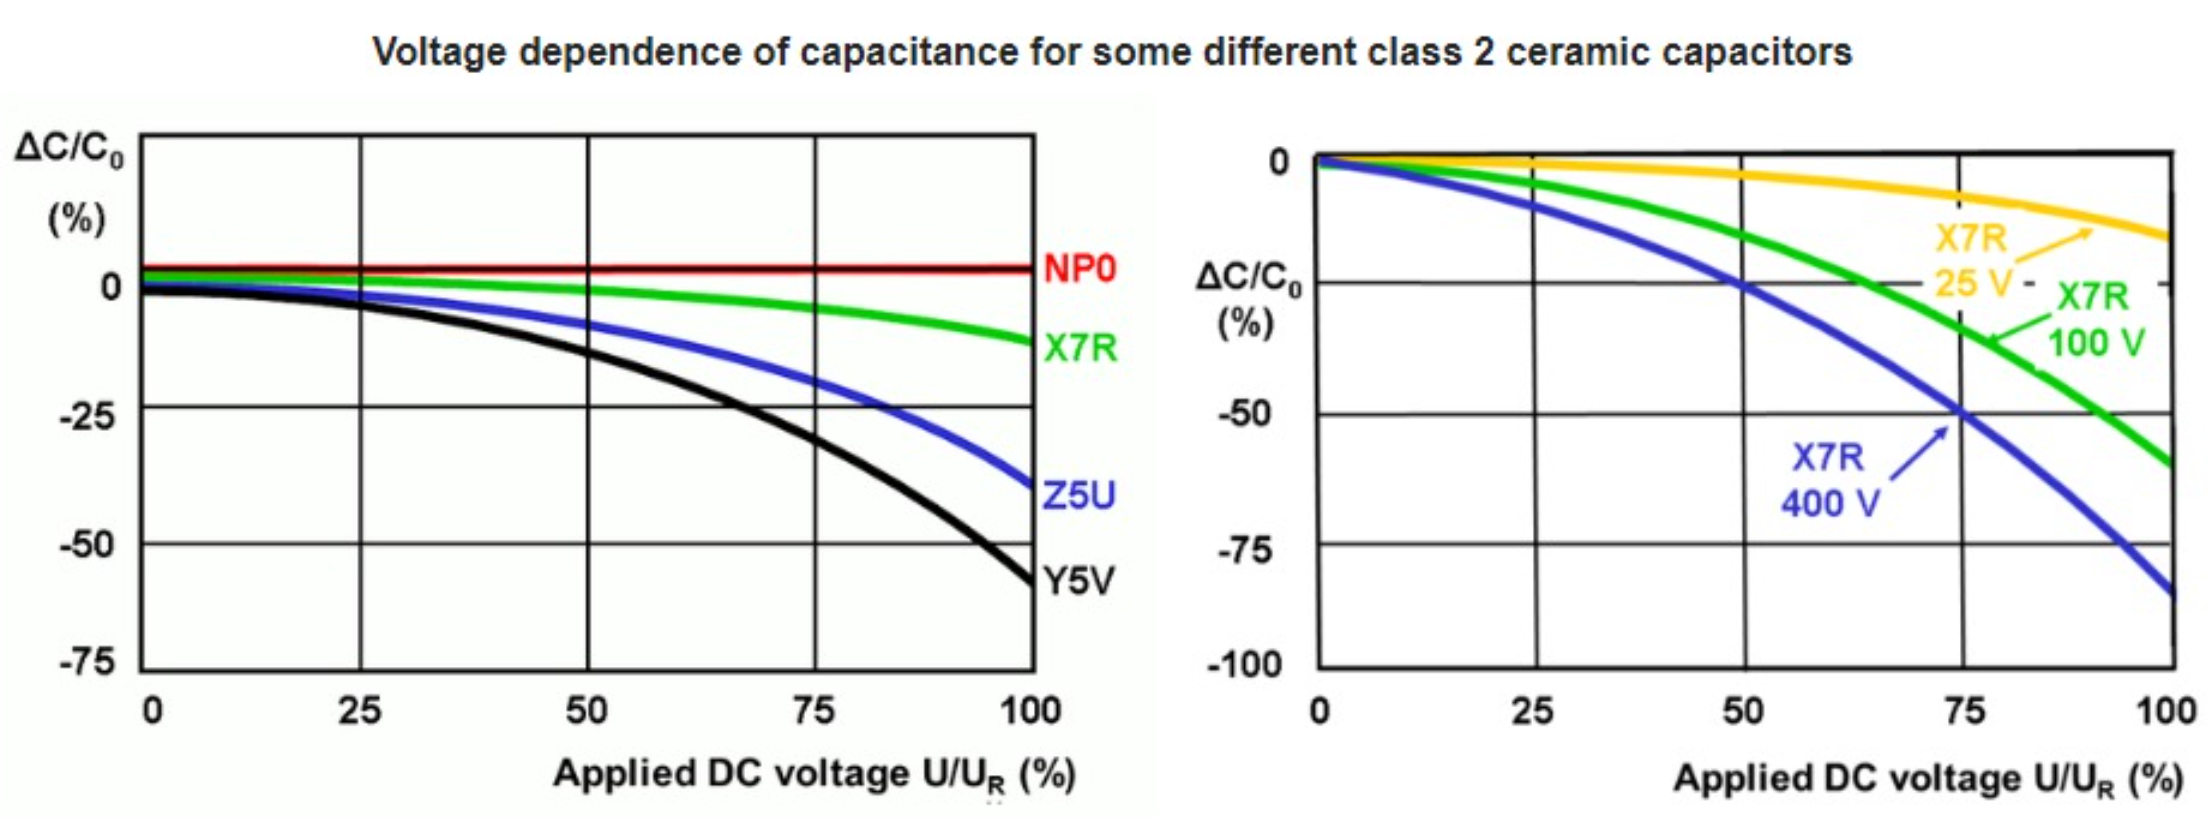
\includegraphics[width=0.8\textwidth]{napiecia_c.png}
    \caption{Spadek pojemności kondensatora ceramicznego wraz ze wzrostem napięcia \cite{st:capacitors}}
    \label{fig:napiecia_c}
\end{figure}

Wybrany kondensator jest klasy 2, wykonany z materiału X7R, co oznacza, że jego pojemność spadnie w przybliżeniu o 30\% dla napięcia \SI{220}{\volt}.
Zdecydowano się na zastosowanie 2 kondensatorów o wartości \SI{2.2}{\micro\farad} połączonych równolegle w celu zminimalizowania tętnień napięcia wyjściowego.
Ostatecznie pojemność oszacowana na:
\begin{equation}
    C_{220} = 2 \cdot (1-0.3) \cdot \SI{2.2}{\micro\farad} = \SI{3.08}{\micro\farad}
\end{equation}

Obliczono tętnienia dla dobranych wartości kondensatorów:
\begin{equation}
    \Delta V_{220} = \frac{V_{out}}{2 \cdot \frac{V_{out}}{I_{out}} \cdot C} \cdot \frac{D}{f_{sw}} = \frac{220}{2 \cdot \frac{220}{0.02} \cdot 3.08\si{\micro\farad}} \cdot \frac{0.945}{500000} \approx \SI{ 6.1}{\milli\volt}
\end{equation}

\begin{equation}
    \Delta V_{130} = \frac{V_{out}}{2 \cdot \frac{V_{out}}{I_{out}} \cdot C} \cdot \frac{D}{f_{sw}} = \frac{130}{2 \cdot \frac{130}{0.02} \cdot 3.08\si{\micro\farad}} \cdot \frac{0.908}{500000} \approx  \SI{5.89}{\milli\volt}
\end{equation}

Wartości tętnień jest mniejsza niż założone \SI{0.1}{\volt}, co oznacza, że dobrano odpowiednie wartości kondensatorów.

\subsubsection{Dobór diody}
Oszacowano prąd diody na podstawie wzoru z karty katalogowej:
\begin{equation}
    I_{d} = \frac{I_{out}}{1-D} + \Delta I_{out} = \frac{0.02}{1-0.945} + 0.006 \approx \SI{0.37}{\ampere}
\end{equation}

Dioda powina mieć prąd przewodzenia większy niż \SI{0.4}{\ampere} oraz być diodą szybko przełączającą, by zminimalizować straty w układzie.

Zdecydowano się na zastosowanie diody ES1G firmy Onsemi, 
która jest diodą super szybką, o prądzie przewodzenia \SI{1}{\ampere}, co jest wystarczające dla tego zastosowania.
Dioda ta ma maksymalne napięcie wsteczne \SI{400}{\volt}, co pozwala na bezpieczne zastosowanie w tym układzie.

\subsubsection{Dobór tranzystora}
Można założyć że prąd tranzystora to prąd cewki, czyli \SI{20}{\milli\ampere}.
Zgodnie z kartą katalogową tranzystor powinien mieć następujące parametry:
\begin{itemize}
    \item Napięcie minimalnie drain-source: \SI{250}{\volt}
    \item Jak najmniejszy $R_{DS(on)}$
    \item Prąd przewodzenia większy niż \SI{0.5}{\ampere}
    \item Niskie napięcie progowe $V_{TH}$
    \item Jak najmniejszy ładunek bramki
    \item Wymaganego prąd bramki mniejszego niż \SI{1}{\ampere}
\end{itemize}

Zdecydowano się na zastosowanie tranzystora N-Channel
MOSFET TPH5200FNH firmy Toshiba, który ma następujące parametry:
\begin{itemize}
    \item Napięcie drain-source: \SI{250}{\volt}
    \item $R_{DS(on)}$: \SI{44}{\milli\ohm}
    \item Prąd przewodzenia: \SI{26}{\ampere}
    \item Napięcie progowe: \SI{2}{\volt}
    \item Ładunek bramki: \SI{22}{\nano\coulomb}
    \item Rozpraszana moc: \SI{2.5}{\watt}
\end{itemize}

Średni prąd bramki potrzebny do załączenia tranzystora można obliczyć na podstawie wzoru:
\begin{equation}
    I_{g} = Q_{g} \cdot f_{sw} = \SI{22}{\nano\coulomb} \cdot 500000 = \SI{11}{\milli\ampere}
\end{equation}
Tranzystor ten spełnia wszystkie założenia, a także ma bardzo niskie $R_{DS(on)}$, co pozwala na zminimalizowanie strat w układzie.
Moc wydzielana na tranzystorze można obliczyć na podstawie wzoru:

\begin{equation}
    P_{mos} = I_{l}^2 \cdot R_{DS(on)} = 0.468^2 \cdot 0.044 \approx \SI{0.01}{\watt}
\end{equation}

Moc jest bardzo niska, co oznacza, że tranzystor nie będzie się nagrzewał, a także nie będzie wymagał radiatora.

\subsubsection{Ustawienie napięcia wyjściowego}
Napięcie wyjściowe będzie regulowane, dlatego zdecydowano się na zastosowanie potencjometru cyfrowego włączonego w obwód sprzężenia zwrotnego.
Potencjometr cyfrowy będzie się komunikował z mikrokontrolerem za pomocą magistrali I2C, co pozwoli na programowe ustawianie napięcia wyjściowego,
by regulować jasność lamp.

Wybrano potencjometr cyfrowy MCP4018T-103E/LT firmy Microchip,
który ma 128 poziomów ustawień, co pozwala na dokładne ustawienie napięcia wyjściowego,
wybrano wartość \SI{10}{\kilo\ohm}, co pozwala na uzyskanie odpowiedniego zakresu ustawień napięcia wyjściowego.

Zgodnie z kartą katalogową napięcie na pinie FB powinno wynosić \SI{1.26}{\volt}, napięcie to oznacza, że napięcie wyjściowe jest odpowiednie. 
Po przetestowaniu kilku kombinacji zdecydowano się na zastosowanie następujących rezystorów:
\begin{itemize}
    \item $R_{fb1} = \SI{2.49}{\mega\ohm}$
    \item $R_{fb2} = \SI{14.39}{\kilo\ohm}$
\end{itemize}

Obliczone napięcie na wyjściu dla potencjometru z nastawą \SI{10}{\kilo\ohm}:
\begin{equation}
    V_{out} = 1.26 \cdot (1 + \frac{R_{fb1}}{R_{fb2} + R_{pot}}) = 1.26 \cdot (1 + \frac{\SI{2.49}{\mega\ohm}}{\SI{14.39}{\kilo\ohm} + \SI{10}{\kilo\ohm}}) \approx \SI{130.4}{\volt}
\end{equation}
Obliczone napięcie na wyjściu dla potencjometru z nastawą 0\si{\ohm}:
\begin{equation}
    V_{out} = 1.26 \cdot (1 + \frac{R_{fb1}}{R_{fb2} + R_{pot}}) = 1.26 \cdot (1 + \frac{\SI{2.49}{\mega\ohm}}{\SI{14.39}{\kilo\ohm}}) \approx \SI{220.6}{\volt}
\end{equation}

Uzyskano zakres napięcia wyjściowego od \SI{130.4}{\volt} do \SI{220.6}{\volt}, co jest zgodne z założeniami projektowymi.

\subsubsection{Dobór rezystora ograniczającego prąd}
Układ ma możliwość ustawienia limitu prądu jaki będzie płynąć przez tranzystor,
co jest dodatkowym zabezpieczeniem przed uszkodzeniem tranzystora.

Najpierw obliczono wartość limitu szczytowego prądu przełączania zgodnie z kartą katalogową:
\begin{equation}
    ISW_{limit} = \left(\frac{I_{out}}{1-D}+\frac{D \cdot V_{in}}{2 \cdot f_{sw} \cdot L}\right) = \left(\frac{0.02}{1-0.945}+\frac{0.945 \cdot 12}{2 \cdot 500000 \cdot \SI{180}{\micro\henry}}\right) \approx \SI{0.426}{\ampere}
\end{equation}

Następnie obliczono wartość rezystora ograniczającego prąd zgodnie z kartą katalogową:
\begin{equation}
    R_{sense} = \frac{V_{SENSE} - (D \cdot V_{SENSE} \cdot V_{SL-ratio})}{ISW_{limit}} = \frac{\SI{156}{\milli\volt} - (0.945 \cdot \SI{156}{\milli\volt} \cdot 0.49)}{0.426} \approx \SI{74}{\milli\ohm}
\end{equation}

Następnie sprawdzono warunek na maksymalną wartość rezystora ograniczającego prąd:
\begin{equation}
    R_{sense} < \frac{2 \cdot V_{SL} \cdot f_{sw} \cdot L}{V_{out} - (2 \cdot V_{IN})} = \frac{2 \cdot \SI{92}{\milli\volt} \cdot 500000 \cdot \SI{180}{\micro\henry}}{220 - (2 \cdot 12)} \approx \SI{84}{\milli\ohm}
\end{equation}

Zdecydowano się na zastosowanie rezystora o wartości \SI{75}{\milli\ohm}, który spełnia wszystkie założenia.
Został również dodany kondensator o wartości \SI{10}{\pico\farad} w celu zminimalizowania tętnień napięcia na rezystorze,
oraz rezystor kompensujący \SI{100}{\ohm}. Schemat elektryczny przetwornicy przedstawiono na rysunku \ref{fig:schemat}.
\begin{figure}[H]
    \centering
    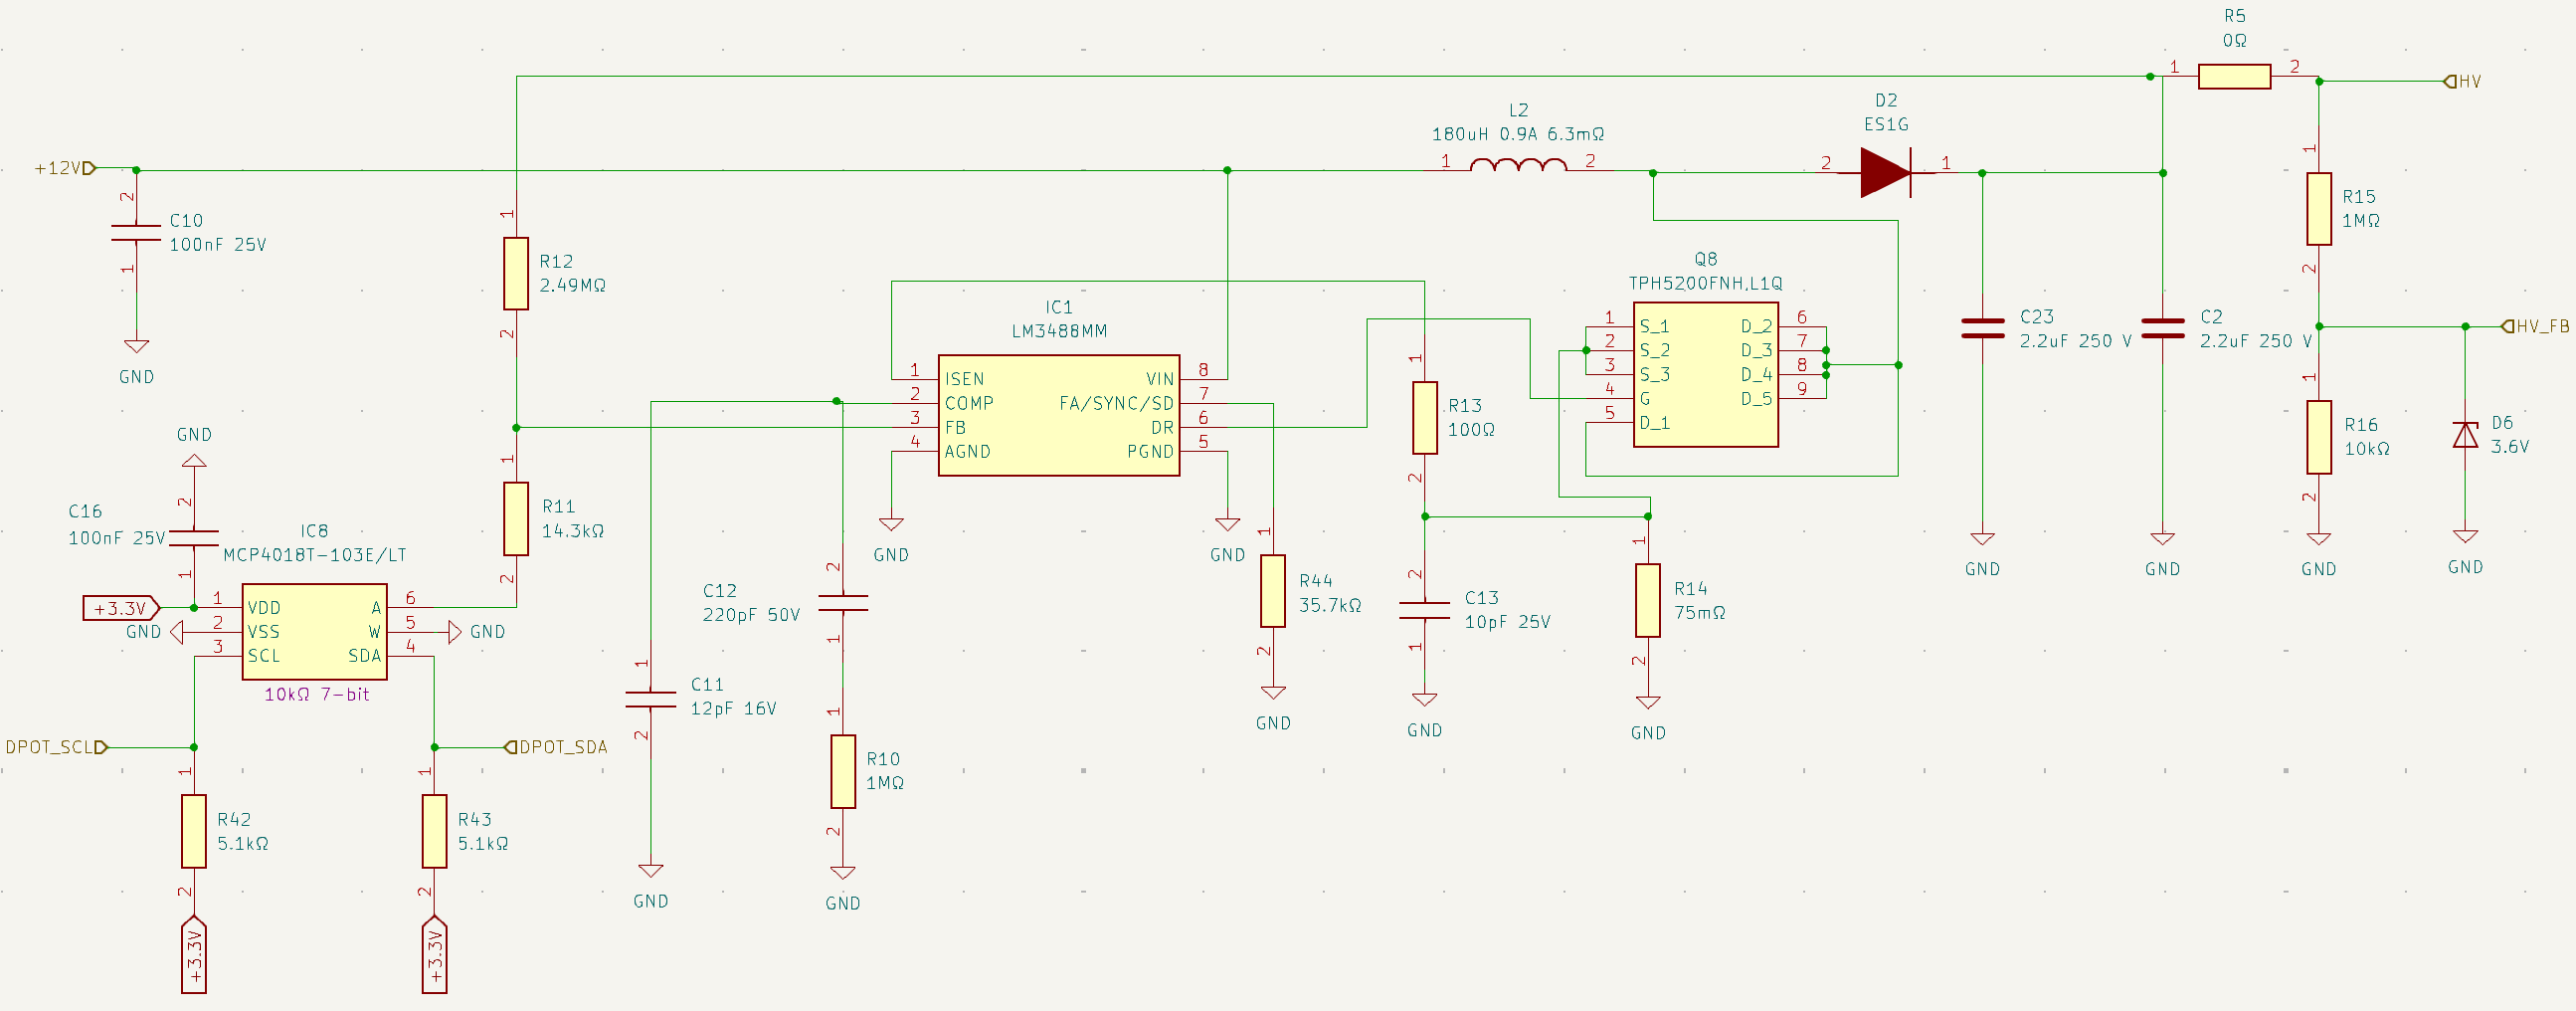
\includegraphics[width=1\textwidth]{schemat.png}
    \caption{Schemat elektryczny przetwornicy \SI{12}{\volt} na wysokie napięcie}
    \label{fig:schemat}
\end{figure}
\end{document}
